
%\setcounter{chapter}{43}
\chapter{How to Write Papers\index{Papers}}
\label{chapter:how_to_write_papers}

\section{Introduction}
An important part of research is communicating your results to others, so we include our thoughts about how to write good papers.  A video presentation of material related to this chapter is \cite{FreemanPapers2020}.

Many graduate students we know feel it is important to coauthor many papers.  While the number of papers a student has can be a rough measure of research productivity, it is our experience as mentors, faculty search committee members, and industrial research managers that {\em only the good papers count}. (We acknowledge that this is not true everywhere, and some institutions simply count papers. But you should still strive to make all your papers good!)  This emphasis is shown in \fig{\ref{fig:impact}}, a plot of made-up data that summarizes our impression, formed over many years, of the relationship between paper quality and its impact on one's career.  Only the really good papers matter for your career.  So it makes sense to learn how to write the best possible paper from any given piece of research work.

\begin{figure}
\centerline{
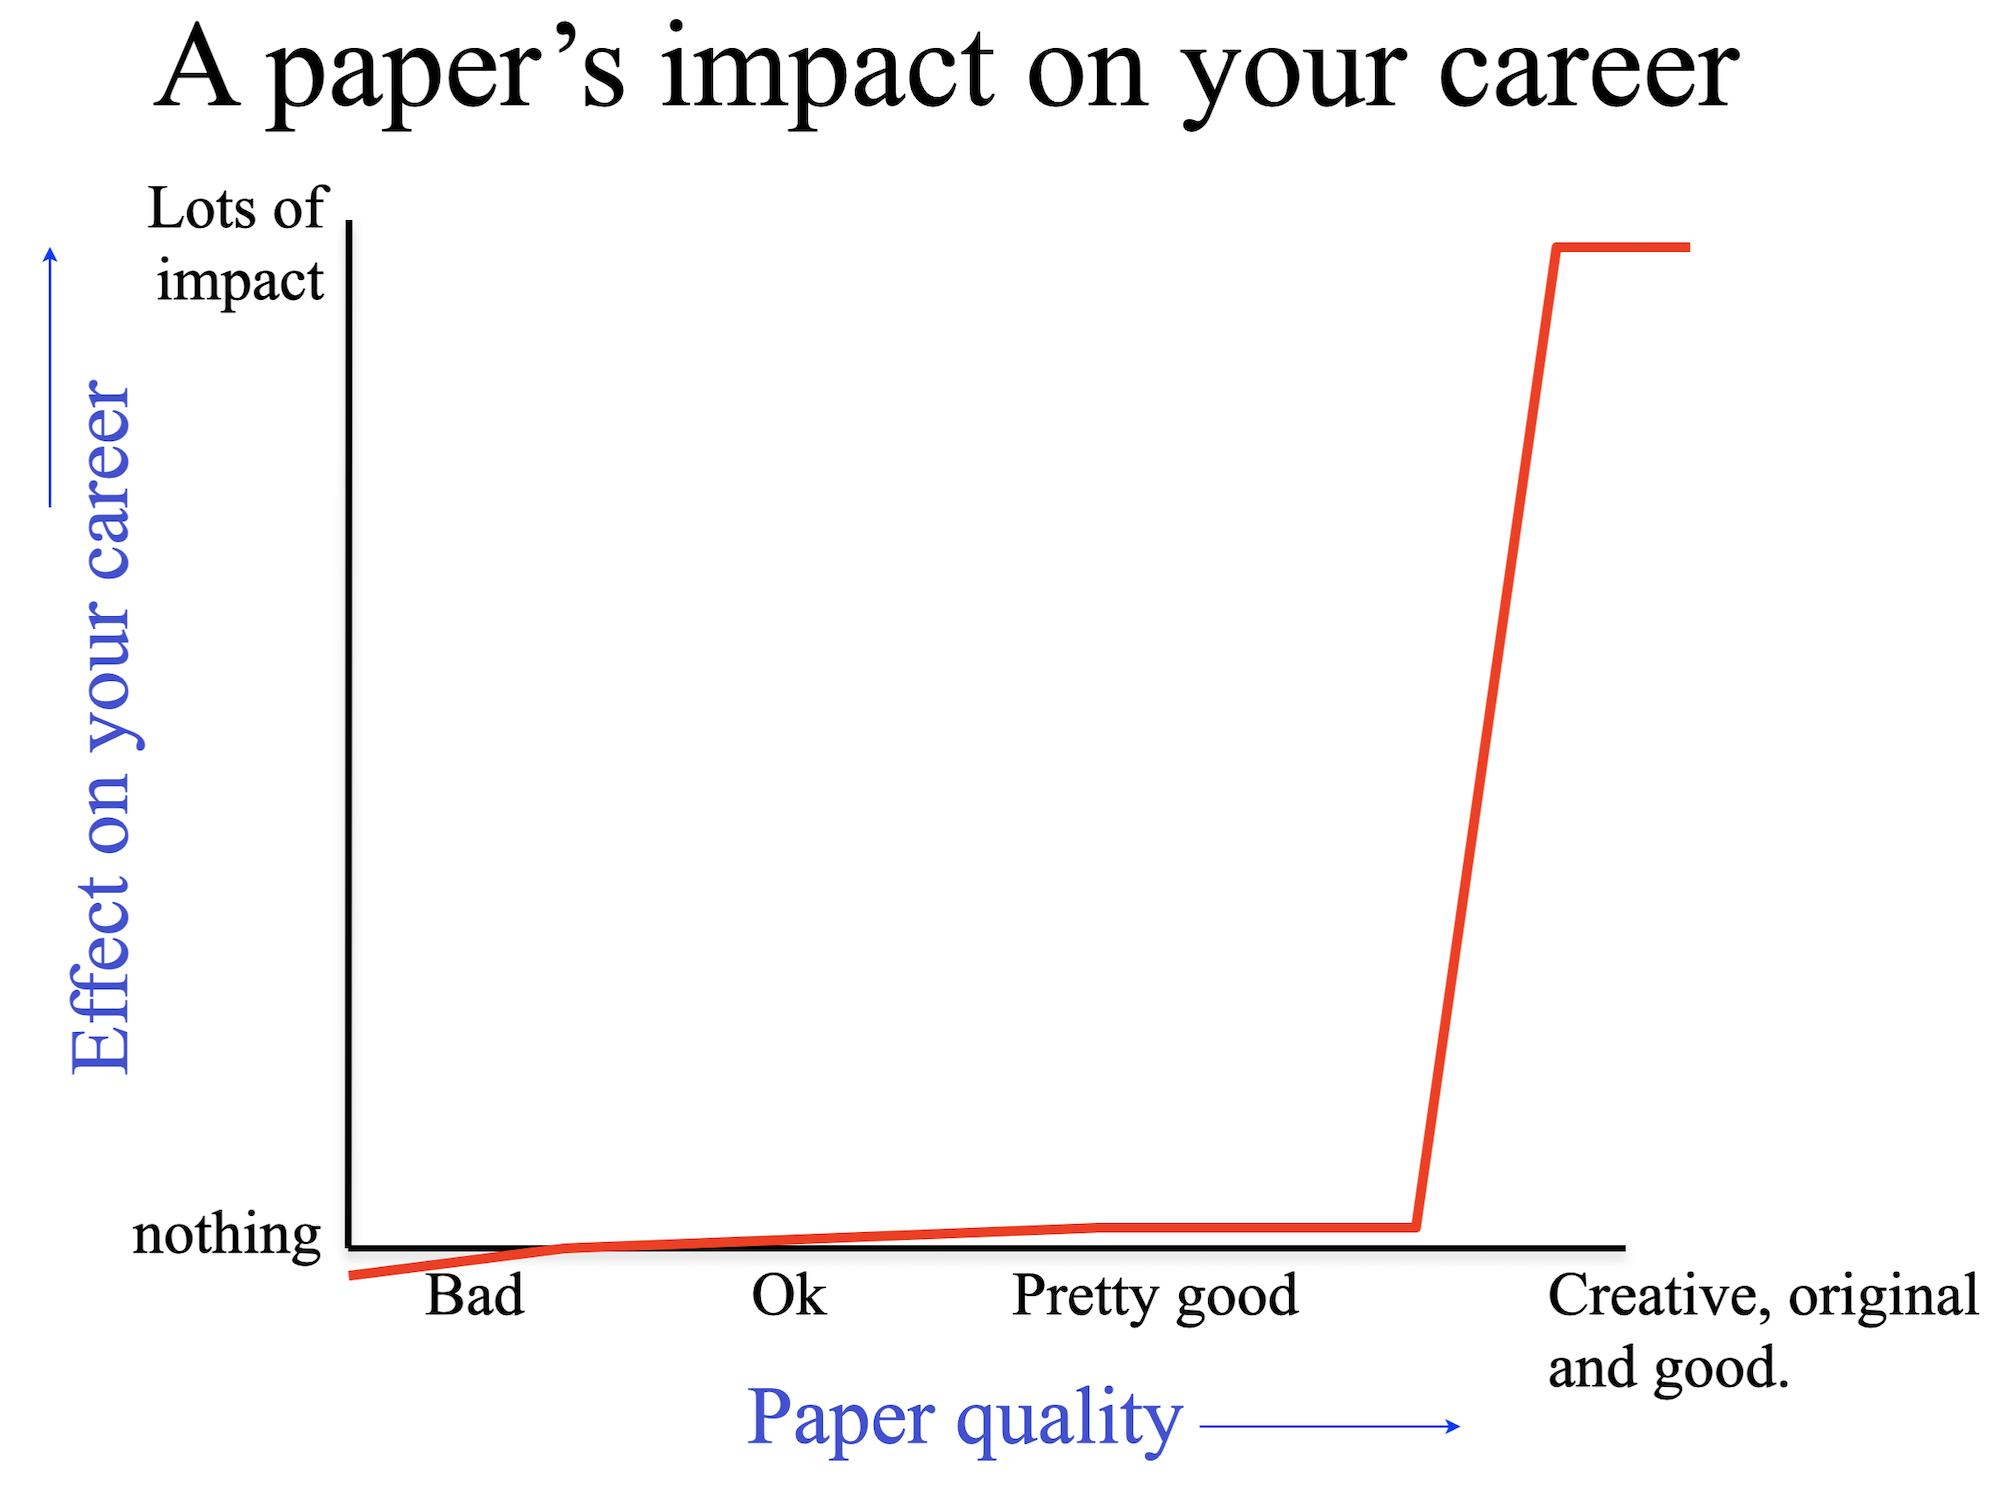
\includegraphics[width=0.60\linewidth]{figures/papers/impact.jpg}}
\caption{Plot of conjectured data showing the impact of a paper on one's career, as a function of paper quality. }
\label{fig:impact}
\end{figure}


\section{Organization}
The Ph.D. thesis advisor of two of us, Prof. Edward Adelson, wrote some good advice in response to a student's question of how to write a good paper \cite{Adelson92}:

\begin{itemize}
\item Start by stating which problem you are addressing, keeping the  
  audience in mind.  They must care about it, which means that sometimes 
  you must tell them why they should care about the problem. 
  
\item Then state briefly what the other solutions are to the problem, and why they aren't satisfactory.  If they were satisfactory, you wouldn't need to  do the work.  

\item Then explain your own solution, compare it with other solutions, and say why it's better.  

\item At the end, talk about related work where similar techniques and experiments have been used, but applied to a different problem.  
\end{itemize}

That structure fits well with a progression of section headings typical of  many conference papers.  As an example, here are the headings from paper \cite{Fergus2006}, coauthored by one of us.  The structure is useful for many research papers:

\begin{tabular}{ll}
1. & Introduction \\
2. & Related work \\
3. & Main idea \\
4. & Algorithm \\
& 4.1 Estimating the blur kernel \\
& \hspace{1cm} 4.1.1 Multiscale approach \\
& \hspace{1cm} 4.1.2 User supervision \\
& 4.2 Image reconstruction \\
5. & Experiments \\
& 5.1 Small blurs \\
& 5.2 Large blurs \\
& 5.3 Images with significant saturation \\
6. & Discussion \\
\end{tabular}





\subsection{The Paper's Introduction}
Regarding paper introductions, Kajiya \cite{Kajiya1993} writes,
``You must make your paper easy to read. You've got to make it easy for anyone to tell what your paper is about, what problem it solves, why the problem is interesting, what is really new in your paper (and what isn't), why it's so neat. And you must do it up front. In other words, you must write a dynamite introduction.''

\subsection{Main Idea}
When appropriate to the paper, it can be very helpful to show a simple example that captures the main idea of the paper.  Here is a figure from a different paper \cite{Simoncelli92} that conveys the main idea very simply.  The paper's main idea was that wavelets lacked important desirable features for an image representation.  \Fig{\ref{fig:wavelet}} shows the failure of a wavelet representation to form a  translation invariant representation.  The top row shows two versions of the same signal, differing only in a one-sample translation.  The bottom three rows show the coefficients of the high-, mid-, and low-frequency bands of a wavelet representation of that signal.  The figure points out in a simple way the drawback of a wavelet representation with aliased subbands that was the focus of the paper:  as the signal translates, the signal representation energy moves to different frequency bands and changes form within the mid-frequency band.


\begin{figure}
\centerline{
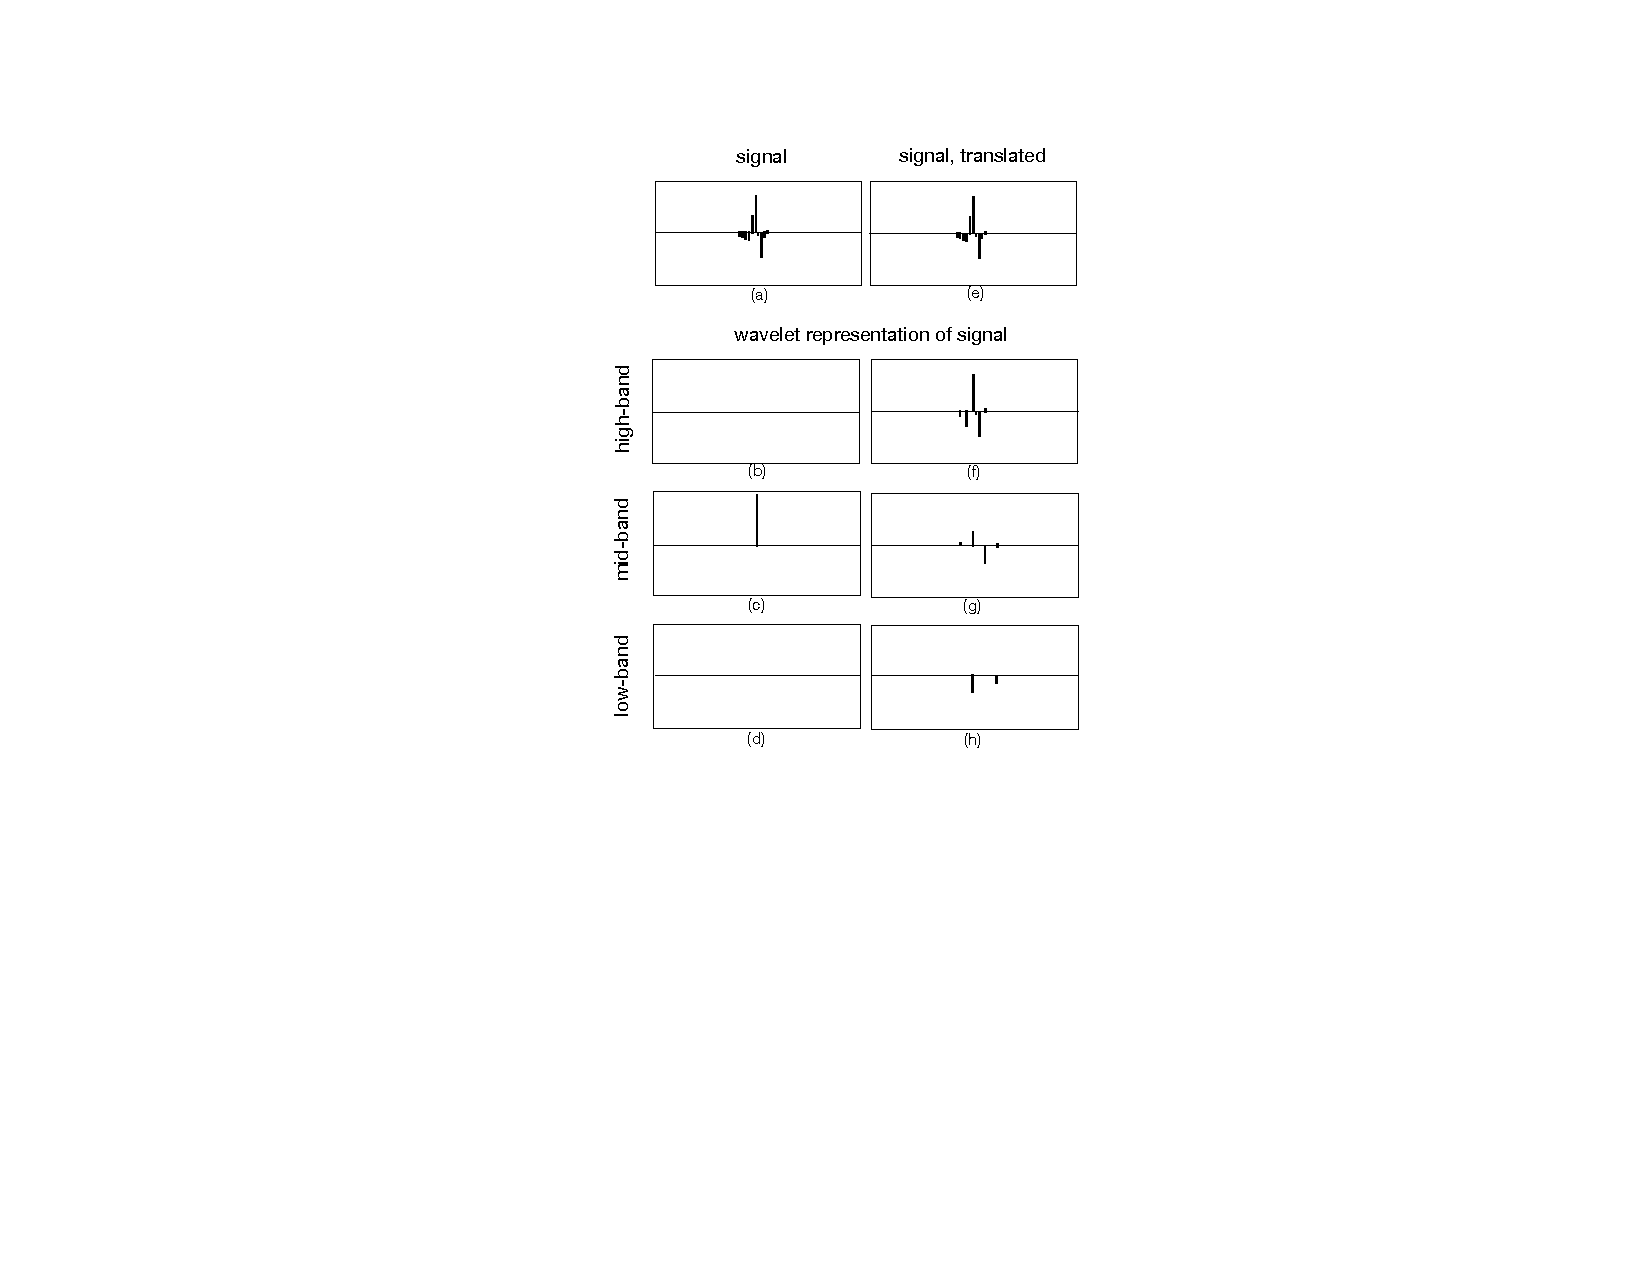
\includegraphics[width=0.65\linewidth]{figures/papers/wavelet2.pdf}}
\caption{Effect of translation on the wavelet representation of a signal  (caption and figure after \cite{Simoncelli92}).  (a) An input signal.  (b-d) The high-, mid-, and low-frequency coefficients within a wavelet subband decomposition.  (e) The same input signal, translated one sample to the right.  (f–h) The decomposition of the shifted signal into the same three bands.  Note the drastic change in the transform coefficients induced by the shift.}
\label{fig:wavelet}
\end{figure}


\subsection{Experimental Results}
In earlier days of computer vision research, good ideas could be presented with only plausibility arguments to support them.  However, 
modern standards require that assertions in a paper be backed up with experimental evidence.  Readers will be expecting a table quantitatively comparing the performance of your algorithm with that of the previous state-of-the-art.  If you are proposing a new task for which there aren't previous benchmarks, you should still compare with an algorithm that solves a related task, noting that the algorithm was designed for a different task.  

\begin{figure}
\centerline{
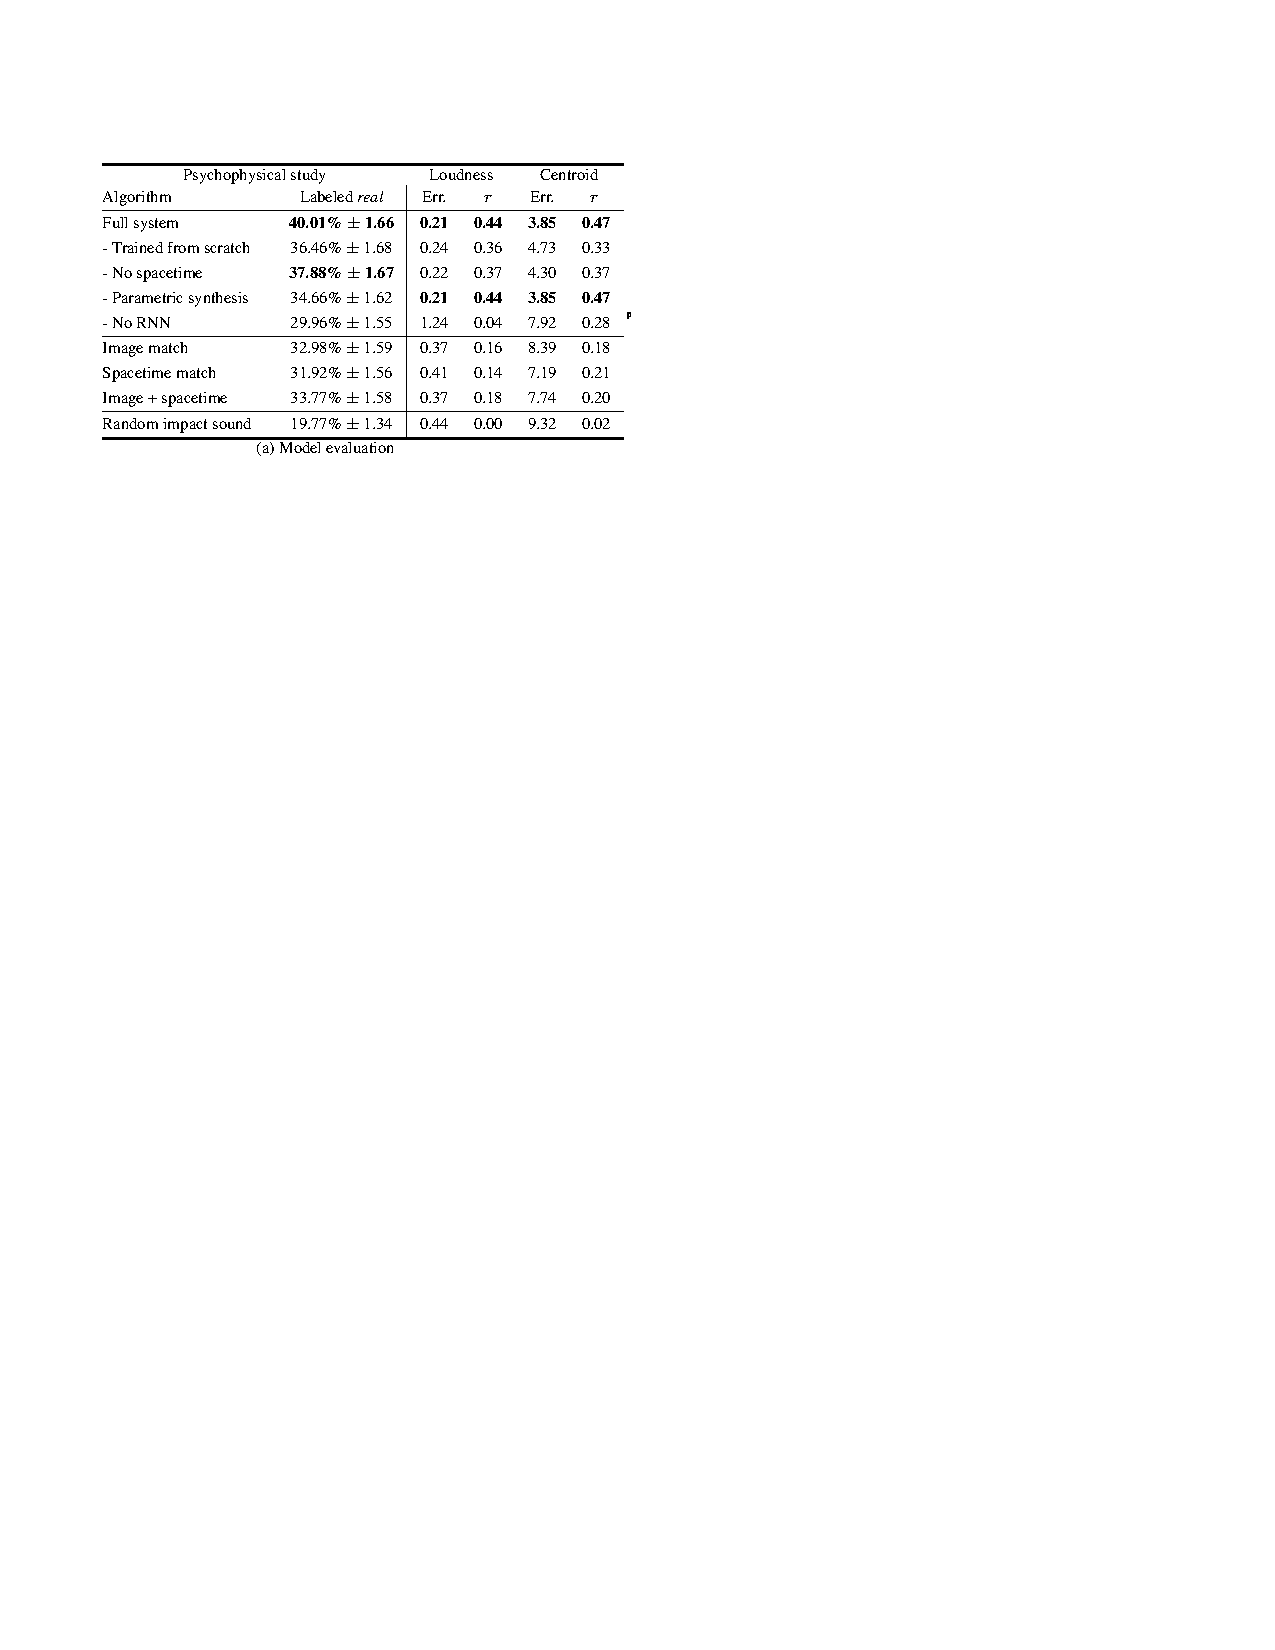
\includegraphics[width=0.75\linewidth]{figures/papers/resultTable.pdf}}
\caption{A prototypical table of results, from \cite{Owens2016}  Rows are different algorithms, or ablations of a favored algorithm. Columns are datasets or tasks, and the numbers indicate performance, with the best performances given in bold. }
\label{resultsTable}
\end{figure}


\subsection{How to End the Paper}

A cautionary note on how {\em not} to end the paper.  Conference papers are often written under deadline pressure, and there is inevitably a list of results that the authors wanted to obtain that have been left uncompleted.  You should resist the temptation to describe the items that were left unfinished in a section on ``Future Work.''  It is hard to imagine a weaker way to end the paper than to enumerate all the things the paper doesn't accomplish, providing a summary of where it falls short.

Instead, the paper can finish with a review what has been presented, emphasizing the contributions.  How has the world changed, now that the reader has read this paper?  What new research directions have been opened up;  what can we do now that we couldn't do before?

\section{General Writing Tips}

Donald Knuth, the author of the classic book series, \booktitle{The Art of Computer Programming}, wrote \cite{Knuth1989},``Perhaps the most important principle of good writing is to keep the reader uppermost in mind:  What does the reader know so far?  What does the reader expect next and why?''

Our mental image is that of a great host, who anticipates every need of their house guest: after you arrive, they say, ``Can I take your coat?  Would you like something to drink?''  At every moment, they know what you might be wanting and how to help you find it.

\subsection{Use Fewer Words}

In \booktitle{The Elements of Style} \cite{Strunk}, Strunk and White write, ``Vigorous writing is concise.  A sentence should contain no unnecessary words, a paragraph no unnecessary sentences, for the same reason that a drawing should have no unnecessary lines and a machine no unnecessary parts.''

To make this point in the context of scientific writing, the following is a paragraph that one of the authors of this textbook wrote with a student.  

\begin{quote}
The underlying assumption of this work is that the estimate of a given
node will only depend on nodes within a patch:  this is a locality
assumption imposed at the patch-level. This assumption can be
justified in case of skin images since a pixel in one corner of the
image is likely to have small effect on a different pixel far away
from itself.  Therefore, we can crop the image into smaller windows,
as shown in Figure 5, and compute the inverse J matrix of the cropped
window.  Since the cropped window is much smaller than the input
image, the inversion of J matrix is computationally cheaper.  Since we
are inferring on blocks of image patches (i.e., ignoring pixels outside
of the cropped window), the interpolated image will have blocky
artifacts.  Therefore, only part of xMAP is used to interpolate the
image, as shown in Figure 5.
\end{quote}
\marginnote{Original text: 149 words.}[0.5in]


While the text above conveys the desired technical information, it describes things in a roundabout way.  The word count is 149. Below, the paragraph has been rewritten to just 88 words without changing its meaning.

\begin{quote}
We assume local influence---that nodes only depend on other nodes
within a patch.  This condition often holds for skin images, which
have few long edges or structures.  We crop the image into small
windows, as shown in Fig. 5, and compute the inverse J matrix of each
small window.  This is much faster than computing the inverse J matrix
for the input image.  To avoid artifacts from the block processing,
only the center region of xMAP is used in the final image, as shown in
Fig. 5.
\end{quote}
\marginnote{Rewritten text conveying the same information: 88 words}[0.5in]

Note that writing more concise text helps your paper in two ways.  First, researchers are typically fighting against a page limit, particularly in conference submissions, so tighter text lets the author say more or add another figure.  Second, concise text is usually clearer and easier to understand.






\subsection{Title, Figure Captions, and Equations}
While we may imagine our reader reading every word of our paper, in our current era of many published papers, most of your readers will probably only skim your paper. We suspect that the engagement of readers with your paper will look something as shown in \fig{\ref{fig:engagement}}.

\begin{figure}
\centerline{
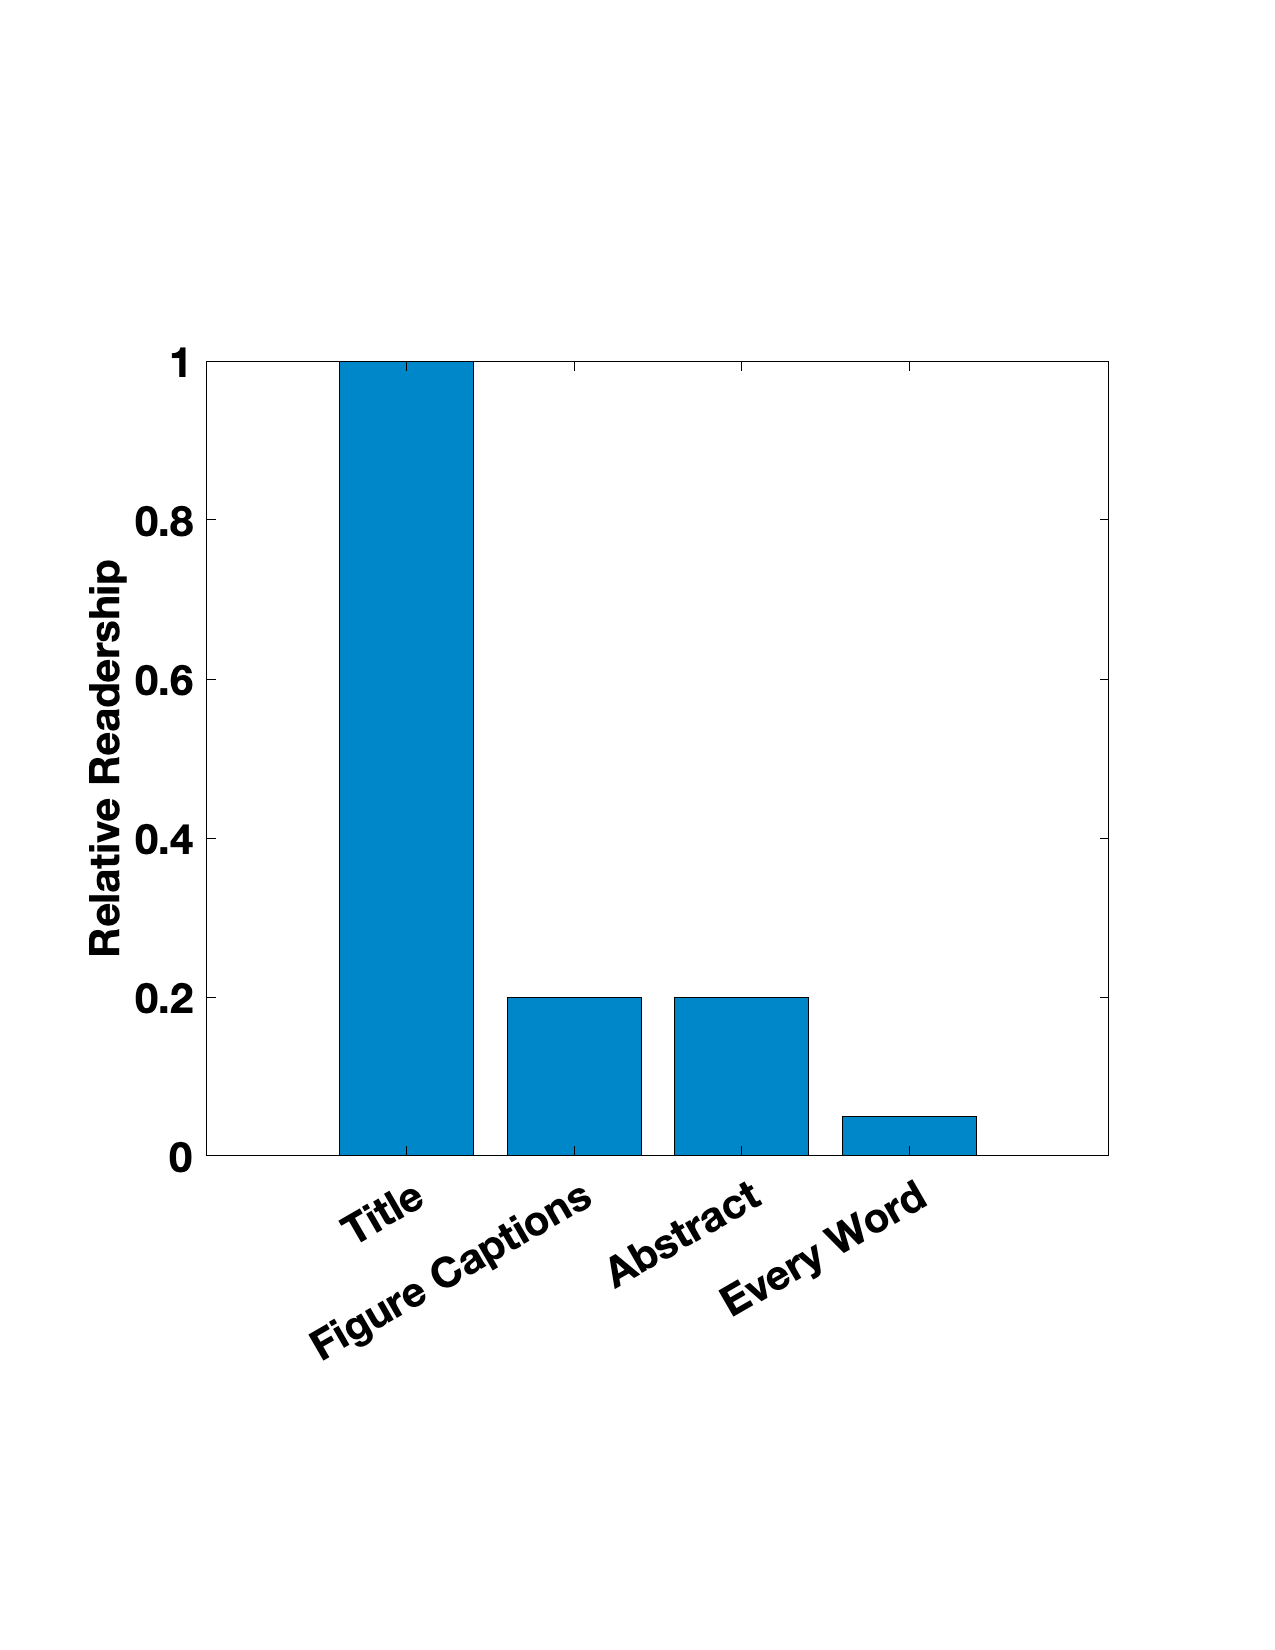
\includegraphics[width=0.50\linewidth]{figures/papers/readership.pdf}}
\caption{The conjectured readership of a computer science paper (conjectured relative amounts).  Many people will read the title, but far fewer will read the abstract or look at the figures.  Fewer still will read every word of the paper.  You should allow readers to access your paper at each level of engagement.}
\label{fig:engagement}
\end{figure}

If only because that is where most of your readership lies, you should write your paper so that readers will learn from it, even at those reduced levels of engagement.  The title should convey the top-level message of the paper.  The figures and their captions should be self-contained and tell the story of the paper.  The abstract should provide a good summary.

A good title can generate attention and interest for the paper.  ``What makes Paris look like Paris'' \cite{doersch2012what}
is a delightful paper, and the title lets the reader see that right away.  In contrast, one of us coauthored a paper called ``Shiftable Multi-scale Transforms.''  While that title is appropriate, it's not catchy.  After the paper was in print, we realized that we should have added the subtitle, ``What's wrong with wavelets?'' --- a catchy phrase that tells the main point of the paper.

Because you can assume that many of the readers of your figure captions will not be reading the full paper, {\em the captions should be self-contained}.  They should point out what readers are supposed to notice about the figure, to help both the full-paper reader and the figures-only reader. \Fig{\ref{fig:shapetime}} shows an example.

\begin{figure}
\centerline{
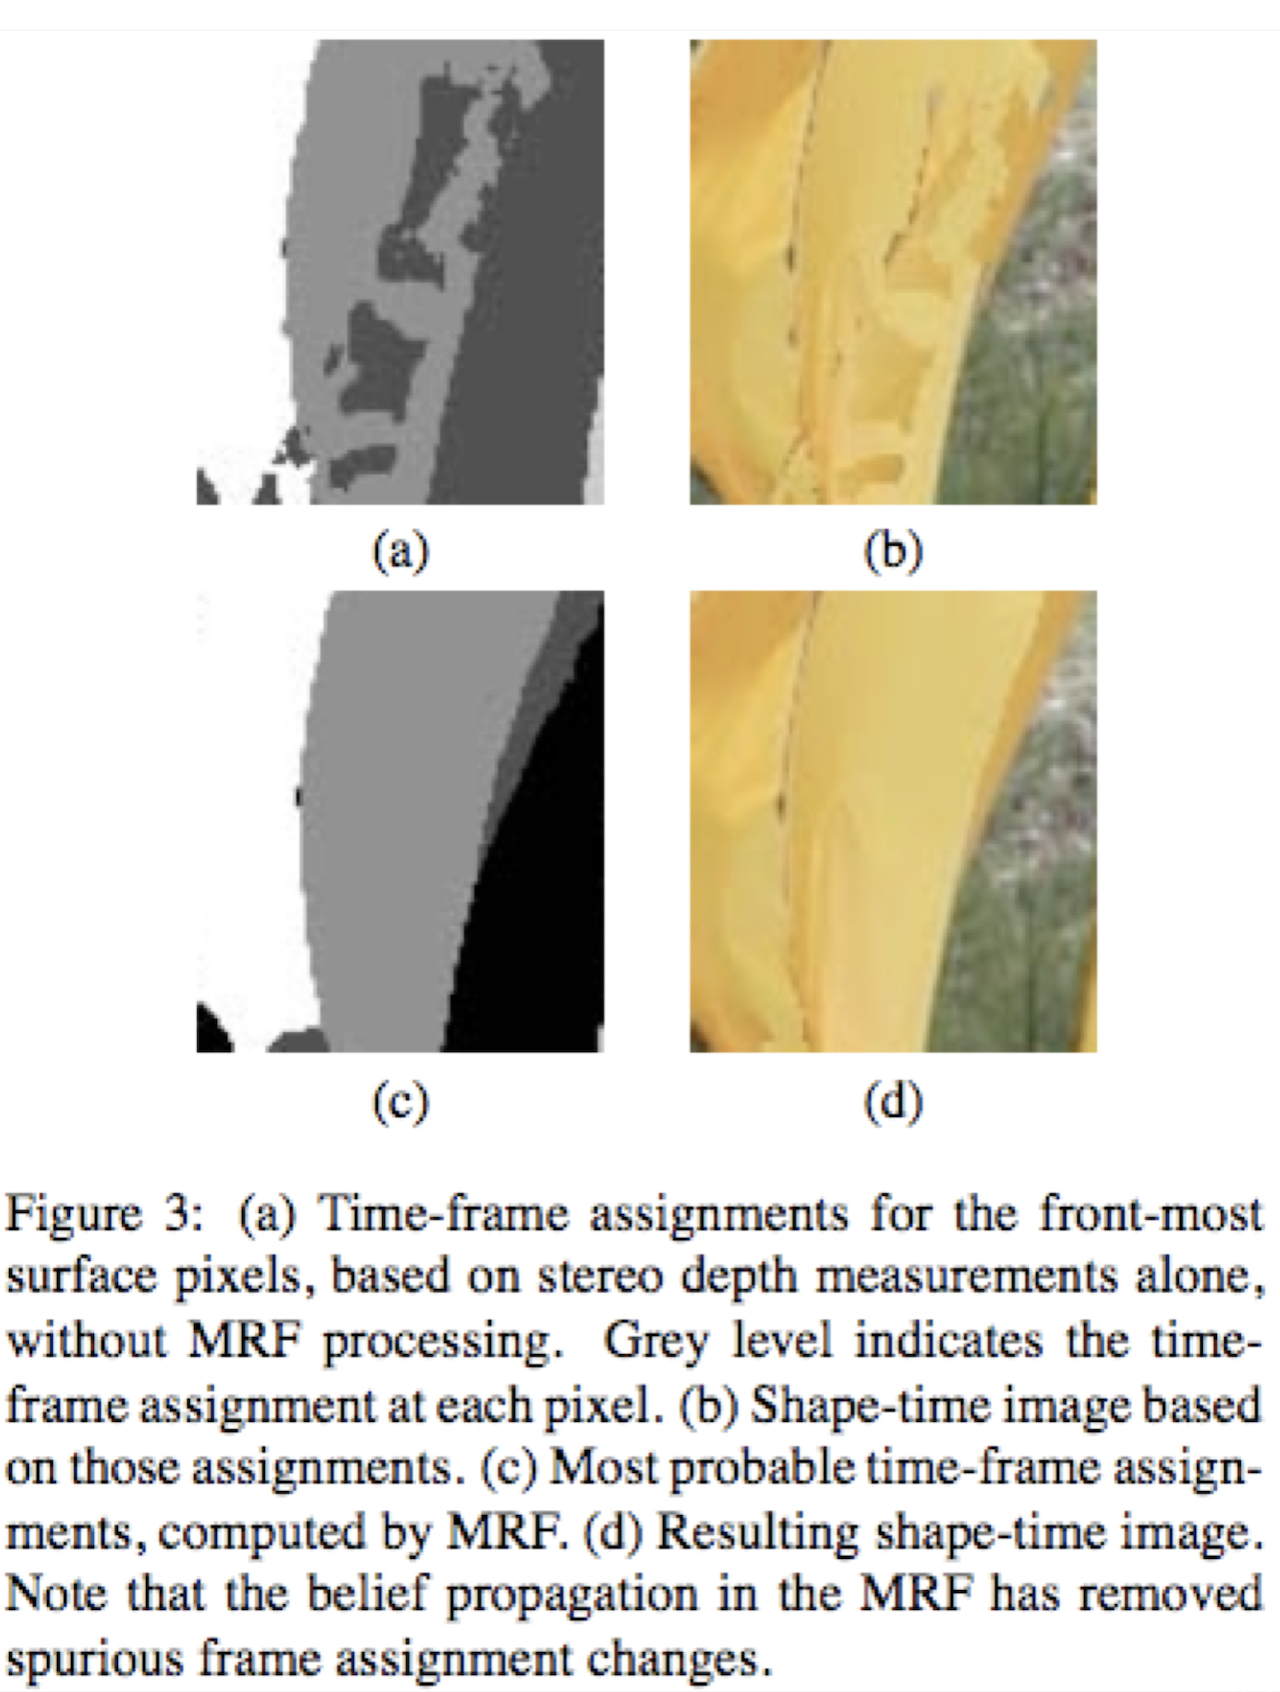
\includegraphics[width=0.55\linewidth]{figures/papers/shapetimeFig.jpg}}
\caption{Figure and caption from \cite{FreemanShapetime}. The caption should be understandable by itself, and should point to what the reader should take away from the figure. }
\label{fig:shapetime}
\end{figure}

Equations interposed with text can pose a challenge to the reader.  Does the reader stop to work through each equation, or continue reading as quickly as if the equation were words?  Knuth \cite{Knuth1989} and Mermin \cite{Mermin1989} both give advice on writing with equations.  Knuth writes,
``{\em Many readers will skim over formulas on their first reading of your exposition.  Therefore, your sentences should flow smoothly when all but the simplest formulas are replaced by `blah' or some other grunting noise.}''

Mermin adds,``{\em When referring to an equation identify it by a phrase as well as a number.  No compassionate and helpful person would herald the arrival of Eq. (7.38) by saying `inserting (2.47 and (3.51 into (5.13)...' when it is possible to say `inserting the form (2.47 of the electric field $E$ and the Lindhard form (3.51) of the dielectric function $\epsilon$ into the constitutive equation (5.13)...' }''


\subsection{Tone}

The tone of your writing is important.  You may feel pressure to oversell, hide drawbacks, and disparage others’ work.  It is in both your short-term and your long-term interest not to succumb to that pressure!  If your work has a shortcoming, it is much better that you point it out than to have someone else do so later.

Papers written from the point of view that ``we're all good researchers, doing our best'' are much more pleasant to read than papers written from the standpoint that everyone else is an idiot.  Note the delightful sentences written by Efros \cite{Efros01} when he was a graduate student, ``{\em A number of papers to be published this year, all developed independently, are closely related to our work.  The idea of texture transfer based on variations of [6] has been proposed by several authors (in particular, see the elegant paper by Hertzmann et al. in these proceedings).  Liang et al. propose a real-time patch-based texture synthesis method very similar to ours.  The reader is urged to review these works for a more complete picture of the field.}''  This generous tone wins over the reader and promotes long-lasting friendships with people who study the same problems you do.

You should develop a reputation for being clear and reliable.  Always convey an accurate impression of the performance of an algorithm.  If something doesn't work in important cases, let the readers know.  In \cite{Fergus2006}, we noted that our deblurring algorithm didn't work for a case where we had been sure it should work for a  maximum a posteriori (MAP)  estimation of the deblurred image. Some years later we learned, and described in \cite{Levin2011}, that we had been wrong to believe that MAP estimation of the deblurred image was feasible.  We were glad we had described our counterintuitive result years before.


\subsection{Author List}

The quality of the papers you write matters so much more than your positions within the author lists of the papers.  If adding more authors will make a paper better, then you should add more authors.   If a collaborator feels they should be an author, but you yourself are not sure, we find it is generally a good idea to trust the collaborator and to add them as a coauthor. It’s much better to be one of many authors on a great paper than to be one of just a few authors on a mediocre paper.

\subsection{Avoiding Rejection}

With the task of rejecting at least three-quarters of the submissions, conference area chairs, who make the acceptance decisions, are grasping for reasons to reject a paper.  Here’s a summary of reasons that are commonly used, and it is best not to provide the area chair with any of these easy reasons to reject your paper:

\begin{itemize}
\item Do the authors not deliver what they promise?
\item Are important references missing (and therefore one suspects the authors not up on the state of the art for this problem)?
\item Are the results too incremental (too similar to previous work)?
\item Are the results believable, with sufficient tests to support the claims?
\item Is the paper poorly written?  
\item Are there mistakes or incorrect statements?
\end{itemize}

As an area chair, the very good and the very bad papers are easy to deal with, and most of the decision-making effort goes to the borderline papers.  One of us writes, ``I find that much of my time is spent dealing with two kinds of borderline papers: cockroaches and  puppies with six toes.''  

``Cockroaches'' have no exciting contributions, but the reviews are ok and the results show incremental improvement to the state of the art.  They're hard to kill (hence the nickname), and maybe two-thirds are accepted as posters, and one-third are rejected.  As an author, it's best to work harder for the fresh results, to bring papers like this out of the cockroach category.

At the other end of the spectrum of borderline papers are ``puppies with six toes.''  These are delightful papers, but with an easy-to-see flaw.  The flaw may not matter (like six toes on a puppy) but makes the paper easy to reject, even though the paper may be fresh and wonderful.  Maybe two-thirds of those papers get rejected, and one-third maybe accepted as posters.  As an author, it may be better to wait for another submission cycle with a paper like this, to remove the easy to spot flaw.  Then the paper might receive an oral presentation at a subsequent conference submission cycle.

\begin{figure}
\centerline{
\sublabelnp{(a) Cockroach}{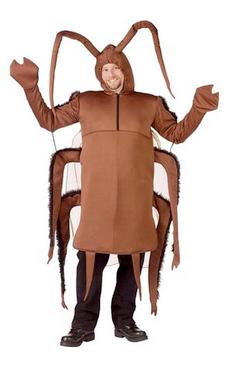
\includegraphics[width=0.23\linewidth]{figures/papers/cockroach.jpg}}
\sublabelnp{(b) Puppy with six toes}{
\includegraphics[width=0.4\linewidth]{figures/papers/puppy6.jpg}}
}
\caption{Borderline papers from an area chair's perspective. (a) The cockroach represents a mundane, hard-to-reject paper with no glaring issues \cite{cockroach}. (b) The six-toed puppy represents delightful paper with some minor, easily spotted flaw, leading to potential rejection \cite{puppy}. }
\label{fig:areachair}
\end{figure}

\section{Concluding Remarks}
The approaches to writing and editing described previously all take time: 
 good writing involves lots of rewriting.  We find that the last days before a paper submission deadline are often better spent improving the structure, presentation, and clarity of the paper than in trying to obtain last-minute improvements to the results.
